% !TeX TS-program = lualatex
% !TeX encoding = UTF-8
% TeX Live Version >=2022
% Diese Vorlage ist lizensiert unter GNU GENERAL PUBLIC LICENSE v3 (29 June 2007)
%
%% Anmerkungen %%
% Diese Vorlage wird weder von der HU-Berlin befürwortet, noch ist sie direkt mit ihr verbunden, autorisiert oder wird auf irgendeine Arte und Weise von ihr gesponsert. 
%
% Vor der Nutzung dieser Vorlage, sollte überprüft werden, ob sie noch den gültigen Richtlinien der HU-Berlin und des entsprechenden Studiengangs entspricht (Aktueller Stand: 2023-07-29 für MA(LIS) Bibliotheks- und Informationswissenschaft)
%
%% Dokumentkonfiguration %%
\directlua{pdf.setminorversion(7)} %Notwendig für korrekte Versionsanzeige wegen LuaLaTeX+pdfx Interaktion 
\documentclass[%
    fontsize=12pt,          %Schriftgröße festlegen
    a4paper,                %Seitenformat auf A4 setzen
    openright,              %Kapitel sollen auf der rechten Seite beginnen
    twoside=semi,           %Zweiseitiges Layout ohne abwechselnde Ränder
    headsepline,            %Trennlinie unterhalb des Headers hinzufügen
    titlepage=firstiscover, %\maketitle als Titelseite anzeigen
    numbers=noenddot,       %Nummerierung nach ISO 2145
    bibliography=totoc,     %Bibliographie zum Inhaltsverzeichnis hinzufügen
    listof=totoc,           %Abbildungs- und Tabellenverzeichnis im Inhaltsverzeichnis
    captions=tableheading,  %Setzt Formatierung für Tabellenüberschriften
    toc=index,              %Index zum Inhaltsverzeichnis hinzufügen
    colorlinks,             %Farbige Links (für Online-Veröffentlichung)
    %hidelinks,              %Versteckte Links (für Druck-Veröffentlichung)
    pdfa,                   %PDF/A Voreinstellungen
    %twocolumn,              %Für zweispaltige Darstellung
    %draft,                  %Auskommentieren für den Entwurfsmodus
    %final                   %Auskommentieren für den endgültigen Druck
    ]{scrbook}              %Verwendung der KOMA-Script book-Klasse

%% Dokumentpaketeausschluss
\PreventPackageFromLoading{fontenc,lmodern} %Sicherstellen dass Standardfonts nicht geladen werden

%% Dokumentpakete
%\usepackage{showframe}%Anzeige der Layout-Boxen
\usepackage{lipsum}   %Generierung von Dummy-Text
\usepackage[a-2b,mathxmp]{pdfx} %PDF/A-2b erzeugen
\usepackage[automark,draft=false]{scrlayer-scrpage} %Detaillierte Konfiguration von Kopf- und Fußzeilen
\usepackage[main=ngerman,british]{babel}%Sprache auf Deutsch setzen
\usepackage{fontspec}                   %LuaLaTeX Standard-Fontpackage
\usepackage{amsmath}                    %Erweiterte Mathematik
\usepackage{unicode-math}               %Unicode-Mathematikmodus erzwingen
    \setmainfont{TeX Gyre Termes}       %Allgemeine Schriftart setzen
    \setmathfont{TeX Gyre Termes Math}  %Mathematische Schriftart setzen
\usepackage{xcolor}   %Verbessertes Farbmanagement
\usepackage[%
    english=british,  %Anführungszeichen für Englisch auf britischen Stil setzen
    autostyle=true    %Anführungszeichen automatisch gemäß Sprache setzen
    ]{csquotes}       %Automatische Formatierung von Anführungszeichen
%\usepackage[%% DEKOMMENTIERE DIES FÜR AUTOR-JAHR ZITATE
    backend=biber,          %Backend auf biber setzen
    style=authoryear-comp,  %Zitierstil (kompakt, Autor-Jahr) setzen
    natbib=true,            %Kompatibilitätsmodus für natbib-Befehle
    doi=true                %Fügt DOI zu Typen hinzu, die sonst keine anzeigen würden
    ]{biblatex}             %Verwendung der Bibliographie
    \AtBeginRefsection{\GenRefcontextData{sorting=ynt}} %Sortierung für Bibliographie festlegen
    \AtEveryCite{\localrefcontext[sorting=ynt]} %Sortierung für Verweise festlegen
    % Anmerkung: Einzeleinstellung notwendig, da sonst Bibliografie nach Jahr sortiert %Dekommentiere diese Linie für Autor-Jahr Zitate
\usepackage[%% DEKOMMENTIERE DIES FÜR NUMERISCHE ZITATE
    backend=biber,      %Backend auf biber setzen
    style=numeric-comp, %Zitierstil (kompakt, Numerisch) setzen
    natbib=true,        %Kompatibilitätsmodus für natbib-Befehle
    sorting=none,       %Eliminiert automatische Sortierung der Einträge
    sortcites=true,    %Sortiert cites Kommandos
    doi=true            %Fügt DOI zu Typen hinzu, die sonst keine anzeigen würden
    ]{biblatex}         %Verwendung der Bibliographie %Dekommentiere diese Linie für numerische Zitate
\usepackage[%
    nameinlink, %Präfix in den Verlinkungen der Referenzen anzeigen
    ngerman,    %Sprache auf Deutsch setzen; unabhängig von Babel erforderlich
    capitalise, %Erster Buchstabe groß (nur wichtig für Englisch)
    noabbrev,   %Deaktiviert Abkürzungen wie Abb. für Abbildung
    ]{cleveref} %Automatische Präfix-Referenzierung
\usepackage[usetransparent=true]{svg} %Erlaubt Inkludierung von SVG Dateien
\usepackage{setspace}                  %Zeilenabstand festlegen
\usepackage{caption}                   %Anpassung der Beschriftungsformatierung
    %\captionsetup[table]{skip=10pt}    %Abstand zwischen Tabelle und Unterschrift
    \captionsetup{labelfont=bf} %Unterschrift in Fettschrift setzen
\usepackage{booktabs} %Bessere Tabellenästhetik
\usepackage{tabularx} %Tabellen mit Zeilenumbruch
\usepackage{array}    %Tabellenfeineinstellungen
\usepackage{multirow} %Tabellenzeilen kombinieren
\usepackage{multicol} %Mehrspaltige Dokumentdarstellung
\usepackage{adjustbox}%Bessere Version von \resizebox
\usepackage{glossaries-extra}%Abkürzung- und Begriffverwaltung
\usepackage{siunitx}  %Bessere Einheitenimplementation
\usepackage{pgfplots} %Akademische Diagramme
    \pgfplotsset{compat=1.18}
\usepackage{tikz}     %Erweiterte Zeichnungs- und Grafikkapazitäten
\usepackage{pdfpages} %Einbinden von PDF-Dateien

%% Neue Befehle und Variabeln
\DeclareNameFormat{labelname:poss}{% Based on labelname from biblatex.def
  \nameparts{#1}% Not needed if using Biblatex 3.4
  \ifcase\value{uniquename}%
    \usebibmacro{name:family}{\namepartfamily}{\namepartgiven}{\namepartprefix}{\namepartsuffix}%
  \or
    \ifuseprefix
      {\usebibmacro{name:given-family}{\namepartfamily}{\namepartgiveni}{\namepartprefix}{\namepartsuffixi}}
      {\usebibmacro{name:given-family}{\namepartfamily}{\namepartgiveni}{\namepartprefixi}{\namepartsuffixi}}%
  \or
    \usebibmacro{name:given-family}{\namepartfamily}{\namepartgiven}{\namepartprefix}{\namepartsuffix}%
  \fi
  \usebibmacro{name:andothers}%
  \ifnumequal{\value{listcount}}{\value{liststop}}{'s}{}}
\DeclareFieldFormat{shorthand:poss}{%
  \ifnameundef{labelname}{#1's}{#1}}
\DeclareFieldFormat{citetitle:poss}{\mkbibemph{#1}'s}
\DeclareFieldFormat{label:poss}{#1's}
\newrobustcmd*{\posscitealias}{%
  \AtNextCite{%
    \DeclareNameAlias{labelname}{labelname:poss}%
    \DeclareFieldAlias{shorthand}{shorthand:poss}%
    \DeclareFieldAlias{citetitle}{citetitle:poss}%
    \DeclareFieldAlias{label}{label:poss}}}
\newrobustcmd*{\posscite}{%
  \posscitealias%
  \textcite}
\newrobustcmd*{\Posscite}{\bibsentence\posscite}
\newrobustcmd*{\posscites}{%
  \posscitealias%
  \textcites} %\posscite-Befehl für besitzanzeigende Zitate im Englischen einbinden
\newcommand{\programme}[1]{\def\programmevar{#1}}
\newcommand{\degreecontext}[1]{\def\degreecontextvar{#1}}
\newcommand{\degree}[1]{\def\degreevar{#1}}
\newcommand{\faculty}[1]{\def\facultyvar{#1}}
\newcommand{\institute}[1]{\def\institutevar{#1}}
\newcommand{\firstsupervisor}[1]{\def\firstsupervisorvar{#1}}
\newcommand{\secondsupervisor}[1]{\def\secondsupervisorvar{#1}}
\newcommand{\keywords}[1]{\def\keywordsvar{#1}}
\newcommand{\languagemetadata}[1]{\def\languagevar{#1}}
\makeatletter
\def\subjectvar{\@subject}
\def\authorvar{\@author}
\def\titlevar{\@title}
\def\subtitlevar{\@subtitle}
\makeatother

\makeatletter
\def\mkfilename#1{%
  \if\relax\detokenize\expandafter{#1}\relax\else#1/\fi}
\AddToHook{include/before}%
  {\IfFileExists{\mkfilename\CurrentFilePath\CurrentFile}{}
     {\GenericError{}{Error: File \mkfilename\CurrentFilePath\CurrentFile.tex not found!}{\@gobble}{}}}
\makeatother

%% Formatierung
\RedeclareSectionCommand[%
    afterindent=false,%Eliminiert Einzug des ersten Paragrafen
    beforeskip=0pt%Eliminiert vertikalen Einzug vor dem Titel
    ]{chapter}%Eliminiert vertikalen Einzug vor Kapitel
\makeatletter
\def\ifdraft{\ifdim\overfullrule>\z@
  \expandafter\@firstoftwo\else\expandafter\@secondoftwo\fi}
\makeatother
\ifdraft{\usepackage{showframe}}{}%Fügt Layoutboxen zum Draft-Modus hinzu
\makeatletter
  \renewcommand{\@pnumwidth}{2em}
  \renewcommand{\@tocrmarg}{3em}
\makeatother %Mehr Platz für Figure-/Table-Nummerierung und Seitenangabe in Verzeichnissen
%% Change Link Colors
\def\tmp#1#2#3{%
  \definecolor{Hy#1color}{#2}{#3}%
  \hypersetup{#1color=Hy#1color}}
\tmp{link}{HTML}{800006}
\tmp{cite}{HTML}{2E7E2A}
\tmp{file}{HTML}{131877}
\tmp{url} {HTML}{8A0087}
\tmp{menu}{HTML}{727500}
\tmp{run} {HTML}{137776}
\def\tmp#1#2{%
  \colorlet{Hy#1bordercolor}{Hy#1color#2}%
  \hypersetup{#1bordercolor=Hy#1bordercolor}}
\tmp{link}{!60!white}
\tmp{cite}{!60!white}
\tmp{file}{!60!white}
\tmp{url} {!60!white}
\tmp{menu}{!60!white}
\tmp{run} {!60!white} %Bessere Standardfarben für Hyperlinks
%% This TeX-file sets most blank pages to contain an 'intentionally left blank' text
\newcommand*{\emptypageline}{THIS PAGE INTENTIONALLY LEFT BLANK}
\newcommand*{\blankpage}{%
  \par\vspace*{\fill}%
  {\centering\MakeUppercase{\emptypageline}\par}
  \vspace{\fill}%
}
%
\makeatletter
\renewcommand*{\cleardoubleoddstandardpage}{%
  \clearpage
  \if@twoside
    \ifodd\c@page
    \else
      \blankpage
      \thispagestyle{empty}%
      \newpage
      \if@twocolumn\hbox{}\newpage\fi
    \fi
  \fi
}
\def\@endpart{%
  \clearpage
  \if@twoside
    \ifodd\c@page
    \else
      \blankpage
      \thispagestyle{empty}%
      \newpage
      \if@twocolumn\hbox{}\newpage\fi
    \fi
  \fi
}
\makeatother %Leere Seiten mit Absichtlich-Text
\renewcommand{\emptypageline}{Diese Seite wurde absichtlich leer gelassen} %Diesen Wert neu definieren, um die gewünschte Meldung anzuzeigen
\recalctypearea %Passt den Textbereich an Einstellungen an

%% Dokumentmetadaten %%
\subject{Thema}
\title{Haupttitel der MA-Arbeit}
\subtitle{Untertitel der MA-Arbeit}
\author{Vorname Nachname}
\date{Abgabedatum}
\publishers{Verlag}
\dedication{Widmung}
\programme{Bibliotheks- und Informationswissenschaft im Fernstudium}
\degreecontext{im Rahmen des Weiterbildenden Masterstudiengangs}
\degree{Masterarbeit}
\faculty{Philosophische Fakultät}
\institute{Institut für Bibliotheks- und Informationswissenschaft}
\firstsupervisor{Prof. Dr. Henry Jekyll}
\secondsupervisor{Prof. Dr. Edward Hyde}
\keywords{Stichwort1, Stichtwort2}
\languagemetadata{de-DE}
%
% PDF Metadaten
\pdfinfo{
  /Author (\authorvar)
  /Title (\titlevar: \subtitlevar)
  /Subject (\subjectvar)
  /Keywords (\keywordsvar)
  /Lang (\languagevar)
}


%% Bibliografie %%
\addbibresource{matter/backmatter/bibliography.bib} %Hauptbibliographieinformationen hinzufügen
%Anmerkung: Das Bibliografieformat muss oben unter Dokumentpakete eingestellt werden

%% Hauptdokument %%
%\includeonly{content/einfuehrung} %Selektive Dokumentgenerierung
\begin{document}
    %% Vorderer Teil
    \frontmatter
        %\makeatletter
\begin{titlepage}
\doublespacing\centering%
\textbf{\Huge\sffamily \@title}\vskip 2.5mm

\textbf{\Large\sffamily \@subtitle}\vfill

{\large Arbeit zum Erreichen des Grades}\\
\textbf{\Large\sffamily\degreevar}\vfill

{\large im Fach}\\
\resizebox{%
      \ifdim\width>\textwidth
        \textwidth
      \else
        \width
      \fi
    }{!}{%
    \textbf{\Large\sffamily\programmevar}}\vfill

{\large eingereicht von}\\
\resizebox{%
      \ifdim\width>\textwidth
        \textwidth
      \else
        \width
      \fi
    }{!}{%
    \textbf{\Large\sffamily \@author}}\vfill

{\large an der}\\
\textbf{\Large\scshape\sffamily Humboldt-Universität zu Berlin}\vfill

\resizebox{%
      \ifdim\width>\textwidth
        \textwidth
      \else
        \width
      \fi
    }{!}{%
    \textbf{\Large\scshape\sffamily\facultyvar}}

\resizebox{%
      \ifdim\width>\textwidth
        \textwidth
      \else
        \width
      \fi
    }{!}{%
    \textbf{\Large\scshape\sffamily\institutevar}}\vfill

\parbox{0cm}{\large%
    \begin{tabbing}
        \textbf{\sffamily1. Gutachter/in:} \= \firstsupervisorvar\\
        \textbf{\sffamily2. Gutachter/in:} \> \secondsupervisorvar
    \end{tabbing}
}\vfill


\enlargethispage{16mm}\textbf{\large\sffamily Berlin, \@date}
\end{titlepage}
\makeatother    %Titelseite ohne Logo
        %\makeatletter
\begin{titlepage}
\doublespacing\centering%
\vspace*{-24.5mm}\noindent\makebox[\textwidth]{\phantom{Vadid Gissnkra}\hspace*{-19mm}\includesvg[height=32.5mm]{matter/titlepage/logo/hu_berlin_logo_text_singleline_black.svg}}

\textbf{\Huge \@title}\vskip 2.5mm

\textbf{\Large \@subtitle}\vfill

{\large Arbeit zum Erreichen des Grades}\\
\textbf{\Large\degreevar}\vfill

{\large im Fach}\\
\resizebox{%
      \ifdim\width>\textwidth
        \textwidth
      \else
        \width
      \fi
    }{!}{%
    \textbf{\Large\programmevar}}\vfill

{\large eingereicht von}\\
\resizebox{%
      \ifdim\width>\textwidth
        \textwidth
      \else
        \width
      \fi
    }{!}{%
    \textbf{\Large \@author}}\vfill

{\large an der}\\
\textbf{\Large\scshape Humboldt-Universität zu Berlin}\vfill

\resizebox{%
      \ifdim\width>\textwidth
        \textwidth
      \else
        \width
      \fi
    }{!}{%
    \textbf{\Large\scshape\facultyvar}}

\resizebox{%
      \ifdim\width>\textwidth
        \textwidth
      \else
        \width
      \fi
    }{!}{%
    \textbf{\Large\scshape\institutevar}}\vfill

\parbox{0cm}{\large%
    \begin{tabbing}
        \textbf{1. Gutachter/in:} \= \firstsupervisorvar\\
        \textbf{2. Gutachter/in:} \> \secondsupervisorvar
    \end{tabbing}
}\vfill


\enlargethispage{16mm}\textbf{\large Berlin, \@date}
\end{titlepage}
\makeatother%Titelseite mit Logo (schwarz-weiß)
        \makeatletter
\begin{titlepage}
\doublespacing\centering%
\vspace*{-24.5mm}\noindent\makebox[\textwidth]{\phantom{Vadid Gissnkra}\hspace*{-19mm}\includesvg[height=32.5mm]{matter/titlepage/logo/hu_berlin_logo_text_singleline_simplified.svg}}

\textbf{\Huge \@title}\vskip 2.5mm

\textbf{\Large \@subtitle}\vfill

{\large Arbeit zum Erreichen des Grades}\\
\textbf{\Large\degreevar}\vfill

{\large im Fach}\\
\resizebox{%
      \ifdim\width>\textwidth
        \textwidth
      \else
        \width
      \fi
    }{!}{%
    \textbf{\Large\programmevar}}\vfill

{\large eingereicht von}\\
\resizebox{%
      \ifdim\width>\textwidth
        \textwidth
      \else
        \width
      \fi
    }{!}{%
    \textbf{\Large \@author}}\vfill

{\large an der}\\
\textbf{\Large\scshape Humboldt-Universität zu Berlin}\vfill

\resizebox{%
      \ifdim\width>\textwidth
        \textwidth
      \else
        \width
      \fi
    }{!}{%
    \textbf{\Large\scshape\facultyvar}}

\resizebox{%
      \ifdim\width>\textwidth
        \textwidth
      \else
        \width
      \fi
    }{!}{%
    \textbf{\Large\scshape\institutevar}}\vfill

\parbox{0cm}{\large%
    \begin{tabbing}
        \textbf{1. Gutachter/in:} \= \firstsupervisorvar\\
        \textbf{2. Gutachter/in:} \> \secondsupervisorvar
    \end{tabbing}
}\vfill


\enlargethispage{16mm}\textbf{\large Berlin, \@date}
\end{titlepage}
\makeatother%Titelseite mit Logo (farbig)
        \chapter{Zusammenfassung}
\lipsum[1-5]
\chapter{Abstract}
\begin{otherlanguage}{british}
\lipsum[1-5]
\end{otherlanguage}      %Deutscher und Englischer Abstract
        \tableofcontents
\listoftables
\listoffigures  %Inhalts-, Tabellen- und Abbildungsverzeichnis
    %
    %% Hauptteil
    \mainmatter
        \chapter{Einführung}
\lipsum[5] \autocite{abbottProfessionalismFutureLibrarianship1998,alaviReviewKnowledgeManagement2001,altenhoenerZukunftFuerSaures2012,batesInformationProfessionsKnowledge2015,batesInformationScienceInvisible1999,begerRechtOeffentlichenZugaenglichmachung2016,bonteAusSachsenWelt2016,bucklandInformationSchoolsMonk2005,bucklandWhatKindScience2012,cuglianaComputationalTurnDigital2022,degkwitzBibliothekZukunftZukunft2016,degkwitzHaveDreamBibliothek2016,dietzeBibliotheksUndInformationswissenschaft1977}

\lipsum[6] 

\lipsum[75]

\section{Unterkapitel}
\lipsum[1-2]
\section{Unterkapitel (Tabellen und Grafiken)}
\lipsum[66]
\begin{table}[!htbp] %%Anmerkung: Diese Tabelle ist komplexer als für die meisten notwendig.
    \centering
    \caption{Ein Beispielstabelle ohne wirklich sinnvollen Inhalt, die aber ästhetisch anspruchsvoll und komplex dargestellt wird.}
    \begin{tabular}{lS[tight-spacing=true]S[scientific-notation=fixed, 
fixed-exponent=-4, round-precision=2, round-mode=places, table-format=1.2e-4,tight-spacing=true]SSS[scientific-notation=fixed, 
fixed-exponent=-4, round-precision=2, round-mode=places, table-format=1.2e-4,tight-spacing=true]S}\toprule
& \multicolumn{3}{c}{Kategorie 1} & \multicolumn{3}{c}{Kategorie 2}
\\\cmidrule(lr){2-4}\cmidrule(lr){5-7}
          & \multicolumn{1}{S}{P1}    & \multicolumn{1}{S}{P2}     & \multicolumn{1}{S}{P3}  & \multicolumn{1}{S}{P4}    & \multicolumn{1}{S}{P5}      & \multicolumn{1}{S}{P6}\\\midrule
Proband 1 & 110 & 1.21e-4 & 13.9 & 158 & 8.7e-5 & 5.6 \\
Proband 2 & 219 & 1.3e-5 & 16.2 & 315 & 1.42e-4 & 18.8 \\
\bottomrule
\end{tabular}
    \label{tab:beispiel}
\end{table}
Siehe \cref{tab:beispiel,fig:hu-logo}.

\noindent\lipsum[66]
\begin{figure}[!htbp]
    \centering
    \includesvg[width=40mm]{matter/titlepage/logo/hu_berlin_logo.svg}
    \caption{Das Logo der Humboldt-Universität zu Berlin, bestehend aus der Illustration der Gebrüder Humboldt mit dem umlaufendem Schriftzug \enquote{Humboldt-Universität zu Berlin}.}
    \label{fig:hu-logo}
\end{figure}

\noindent\lipsum[75]
        \chapter{Beispielkapitel}
\lipsum[1] \autocite{samulowitzBibliothekUndDokumentation2003,sarrafzadehKnowledgeManagementIts2010,saurWissenschaftlicheVerlageVersuch2016,scholzeOpenAccessUnd2016,schrettingerVersuchVollstaendigenLehrbuchs1829,seadleFragilityFutureLibrary2016,siegfriedNutzerbezogeneMarktforschungFuer2014}

\section{Unterkapitel (Struktur)}
\lipsum[3-4]

\subsection{Unter-Unterkapitel}
\lipsum[5-6]

\subsubsection{Unter-Unter-Unterkapitel}
\lipsum[66]

\paragraph{Paragraf}
\lipsum[66]

\subparagraph{Unterparagraf}
\lipsum[75]

\section{Unterkapitel (Mathematische Formel)}
\lipsum[1-5]
\begin{equation}
    \sin x = \sum\limits_{n = 1}^\infty  {\frac{{\left( { - 1} \right)^{n - 1} x^{2n - 1} }}{{\left( {2n - 1} \right)!}}}    
\end{equation}
\lipsum[1]
    %
    %% Hinterer Teil
    {\backmatter%GESCHWEIFTE KLAMMERN NICHT LÖSCHEN! Beeinflusst sonst den Appendix!
        \emergencystretch=1em\printbibliography %Bibliografie mit besserem Umbruch
    }%GESCHWEIFTE KLAMMERN NICHT LÖSCHEN! Beeinflusst sonst den Appendix!
    %
    %% Appendix
    \appendix
    \part*{Appendix}
    \chapter{Beispielappendix}
\lipsum[1-5]
    %% Selbstständigkeitserklärung
    % Wichtig: Ersetze die PDF-Datei mit einer ausgefüllten Variante vor der Abgabe!
    % Wichtig: Die hier beigefügte Datei entspricht der Vorlage des Instituts für Bibliotheks- und Informationswissenschaft. Nutze die Vorlage des entsprechend gültigen Fachbereichs!
    \cleardoubleoddstandardpage
%% Ersetze die folgende PDF-Datei mit einer eigens ausgefüllten Variante
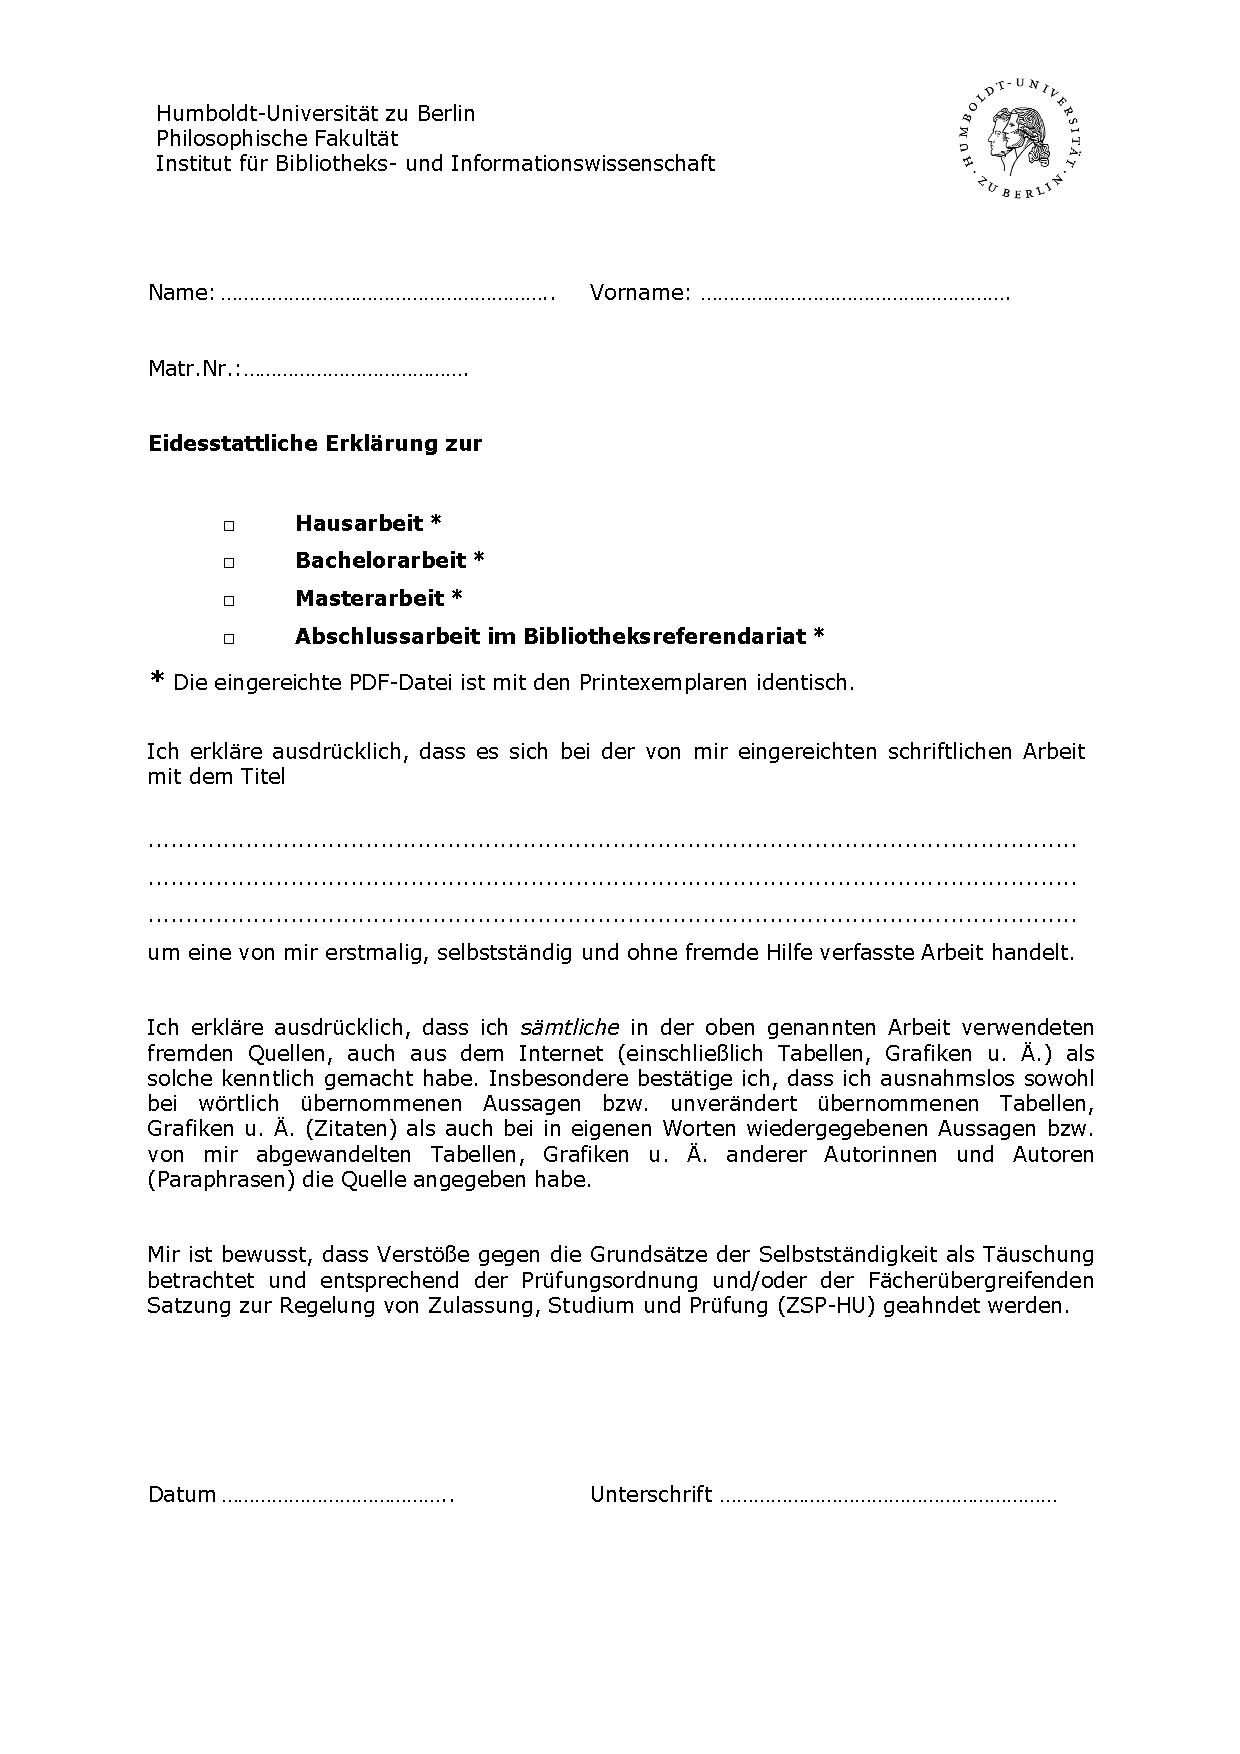
\includepdf[pages=-]{matter/backmatter/selbststaendigkeitserklaerung.pdf}
\end{document}
